\documentclass[11pt,letterpaper]{article}
\usepackage[utf8]{inputenc}
\usepackage{amsmath,amssymb,fullpage,graphicx}
\usepackage{subfigure}
\let\hat\widehat
\let\tilde\widetilde

\begin{document}
\subsection*{Q5-a}

\noindent CDF of $Uniform(0, 1)$, $F_X(x) = \frac{x-a}{b-a} = x$. The qq-plot is presented as $x^{i \star}$ vs $\frac{i}{n+1}$ where $x^{i \star}$ is observed data in $i$th order.

\begin{verbatim}
p_value_dt <- c(0.01, 0.01, 0.02, 0.04, 0.04, 0.05, 0.07, 0.07, 0.10, 0.19,
                0.24, 0.27, 0.34, 0.37, 0.44, 0.50, 0.53, 0.54, 0.55, 0.61,
                0.70, 0.77, 0.80, 0.80, 0.82, 0.94, 0.99)
n <- length(p_value_dt)
expect_qt <- seq(1, n) / (n + 1)  
qqplot(expect_qt, p_value_dt, xlab='Theoratical Quantiles', ylab='Observed Quantiles',
       main='QQ-Plot of P-values')
abline(a=0,b=1)
\end{verbatim}

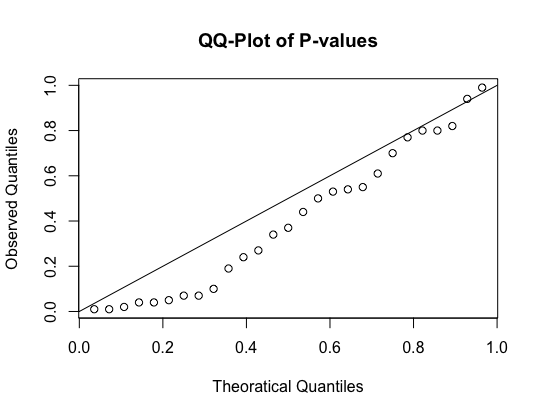
\includegraphics[scale=0.6]{q5-a.png}

\noindent In qq-plot, almost all observed data quantiles are smaller than corresponded theoretical quantiles. Dataset of p-values seem not from $Uniform(0, 1)$, base on the qq-plot. 

\newpage
\subsection*{Q5-b}
\noindent $P(x \in [0, 0.2)) = P(x \in [0.2, 0.4)) = P(x \in [0.4, 0.6)) = P(x \in [0.6, 0.8)) =P(x \in [0.8, 1]) = \frac{1}{5}$, since data are hypothesized from uniform distribution, $F_U(u) = \frac{x-a}{b-a}$.\\

\noindent There are 10 points in first interval, 4 in the second, 5 in the third and fourth, and 3 in the fifth.

\begin{verbatim}
interval_count <- c(10, 4, 5, 5, 3)
> chisq.test(interval_count, p=rep(0.2, 5))

	Chi-squared test for given probabilities

data:  interval_count
X-squared = 5.4074, df = 4, p-value = 0.248
\end{verbatim}

\noindent The chi-square test comes up with p-value of $0.248$, therefore, under the test size $0.05$, observed dataset fail to provide significant evidence against uniform assumption. 


\end{document}